\section{Compiling}

\subsection{Codewarrior Designflow}

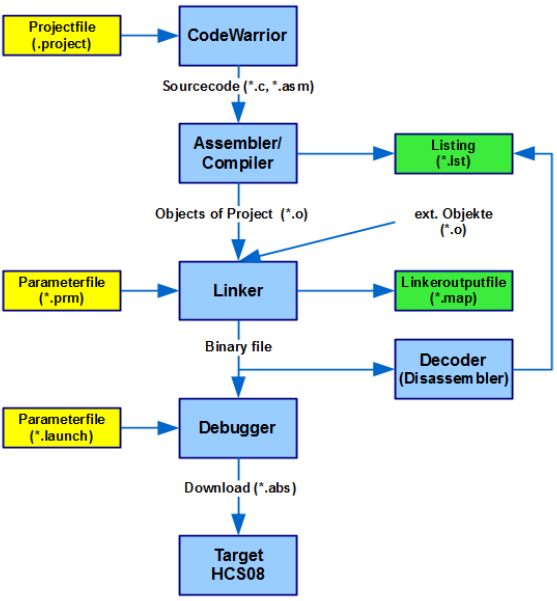
\includegraphics[width=0.5\textwidth]{codewarrior-designflow.png}

\subsection{Programming Language}

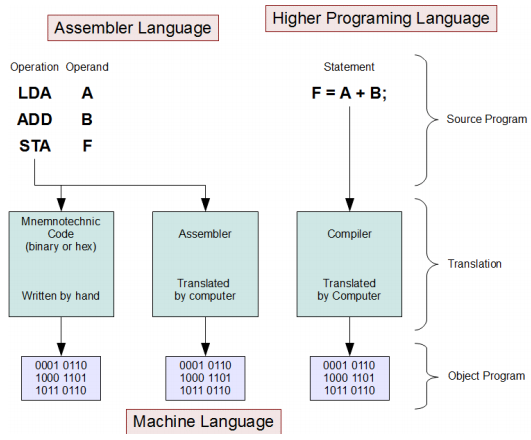
\includegraphics[width=0.5\textwidth]{programming-languages.png}

\textit{High level programming languages are:}

\begin{itemize}
    \item{portable}
    \item{efficient (normaly)}
    \item{Better readable}
    \item{easier to maintain}
\end{itemize}

\textit{
    High level programming languages are usually prefered,
    if enough computational power and memory is available.
}
\\
\textit{
    Assembler is often used, if the application:
}
\begin{itemize}
    \item{is time critical and needs exact timing}
    \item{timing of the high level programming language to unpredictible is}
\end{itemize}

\subsection{Assembler Code-Format}

\begin{tabular}{rllll}
        & \textbf{Label}  & \textbf{Instruction}  & \textbf{Operands} & \textbf{comment} \\
    Ex1 & Limit: & EQU          & \$CD       & ; define limit \\
    Ex2 & Start: & LDA          & \#Limit     & ; load limit \\
\end{tabular}

\textit{
    \textbf{Instruction}: is a command for the processor
} \\
\textit{
    \textbf{Directive}: are instructions that direct the assembler /
    compiler to do something
}

\begin{tabular}{rlll}
        & \textbf{Type} & \textbf{Directed to}  & \textbf{Results in program code} \\
    \hline
    Ex1 & \textbf{Instruction} & Target CPU     & Yes \\
    Ex2 & \textbf{Directive}   & Assembler      & Only indirect \\
        & \textbf{Comment}     & Programmer     & No \\
\end{tabular}

\subsection{Parameter file}

\textit{
    The Parameter file (*.prm) is used for by the Linker. It takes the machine
    code and defines the location on the controller. It is important,
    so that jumps work correctly.
    It contains:
}

\begin{itemize}
    \item{Memory-Map of the Prozessor (Location and size of Flash, RAM, ..)}
    \item{Extra definitions, where which parts of the code on the Controller should be located}
\end{itemize}
